\documentclass[11pt,a4paper]{article}
\usepackage[T1]{fontenc}
\usepackage[utf8]{inputenc}
\usepackage{lmodern}
\usepackage[margin=2.4cm]{geometry}
\usepackage{amsmath,amssymb}
\usepackage{graphicx}
\usepackage{booktabs}
\usepackage{caption}
\usepackage{xcolor}
\usepackage[colorlinks=true,linkcolor=blue!50!black,citecolor=blue!50!black,urlcolor=blue!50!black]{hyperref}
\usepackage{microtype}
\captionsetup{font=small,labelfont=bf}
\graphicspath{{../figures/}}
\newcommand{\Life}{F_{\mathrm{Life}}}

\title{\textbf{Same Mortality, Different Fate:\\ Spatially Clustered Random Deaths in Conway's Game of Life}\\[4pt]
\large Technical research report prepared for supervisor review}
\author{Ali Yi\u{g}it Y\i ld\i z\thanks{High-school student. Project supervised by Prof.\ Levent Suba\c{s}\i{}, Istanbul Technical University (\.{I}T\"{U}). This report has not been reviewed by the supervisor and has not been peer reviewed.}}
\date{Draft of 15 November 2026}

\begin{document}
\maketitle

\begin{abstract}
We study a stochastic version of Conway's Game of Life in which, after every deterministic update, each live cell is removed with probability $\mu$. Two mortality models with the same per-cell removal probability are compared. In the independent model, deaths are uncorrelated. In the clustered model, deaths are generated by thresholding a Gaussian-smoothed random field with correlation width $\sigma$. On periodic $60\times60$ lattices with initial density $p_0=0.35$, independent mortality at $\mu=0.005$ never led to extinction within 3000 updates (0 of 40 runs), whereas clustered mortality with $\sigma=2$ always did (40 of 40, median extinction time 841 updates). This contrast persists for lattice sizes from $L=60$ to $L=200$ and for initial densities from 0.20 to 0.50. The realised fraction of live cells removed per update equals $\mu$ within about 3\% in both models, so the difference is not caused by stronger mortality on average. A control model that reproduces the step-to-step fluctuations in the number of deaths but has no spatial correlation behaves like the independent model at $\mu\le0.005$. Simulations of isolated objects suggest a mechanism. A $2\times2$ block repairs the loss of a single cell in one update, so independent deaths rarely destroy it, while correlated deaths often remove several of its cells at once. All results are for finite lattices and finite observation times.
\end{abstract}

\section{Introduction}

Cellular automata are lattice models in which every site updates its discrete state from the states of nearby sites. Despite their simplicity they show a wide range of collective behaviour, from rapid relaxation to fixed points to irregular, long-lived activity \cite{wolfram1983,wolfram1984}. Conway's Game of Life \cite{gardner1970} is the best known two-dimensional example. Starting from a random configuration it typically evolves through a long transient and then settles into a sparse ``ash'' of still lifes and oscillators. Its statistical properties have been studied for decades, including whether its relaxation is critical \cite{bak1989,bennett1991,blok1999}.

Adding randomness to the Life rule is a natural way to ask how robust this behaviour is. Earlier work introduced a ``temperature'' into the rules \cite{schulman1978}, studied stochastic rules with transitions between a living phase and an extinct phase \cite{monetti1995,nordfalk1996}, and replaced synchronous by partly random updating \cite{blok1999}. Because the empty lattice is absorbing, these models are related to the broad family of non-equilibrium transitions into absorbing states \cite{hinrichsen2000}.

This project began as a sequence of weekly exercises on elementary cellular automata and the Game of Life (Section~\ref{sec:background}). In the last part a simple form of noise was added: after each Life update every live cell dies with probability $\mu$. The student then asked whether it matters \emph{where} these deaths happen. If the probability that a given cell dies is held fixed, but deaths tend to occur together in nearby cells, does the long-time behaviour change? Preliminary simulations in the project notebook suggested a large effect. This report re-examines that observation with matched models, a control model, several lattice sizes, initial densities and correlation widths, and a mechanistic test.

\section{Scientific background}\label{sec:background}

The project notebooks (Weeks 1 to 5) establish the tools used here. They implement elementary cellular automata with periodic boundaries, reproduce Wolfram's qualitative classes for the 256 rules \cite{wolfram1983,wolfram1984}, verify that the number of occupied cells of Rule 90 started from one cell is $N_1(t)=2^{\mathrm{popcount}(t)}$ (a consequence of its additivity \cite{martin1984}), and confirm that perturbations spread no faster than the light-cone bound $R(t)\le t$. They then implement the Game of Life, reproduce the block, beehive, blinker, toad and glider, measure the glider velocity of $1/4$ cell per update in each lattice direction, and use ensembles of random initial grids to show that the late-time density depends non-monotonically on the initial density. All of these results were reproduced exactly when the notebooks were re-executed for this report (see \texttt{VALIDATION\_REPORT.md}).

\section{Research questions and objectives}

\begin{enumerate}
\item How do the late-time density, the activity and the probability of extinction depend on the mortality probability $\mu$ when deaths are independent?
\item At equal mortality probability, does spatial clustering of deaths change the long-time fate of the system?
\item If it does, is the effect caused by the spatial arrangement of deaths or merely by larger fluctuations in their number?
\item Are the observations robust to the lattice size $L$, the initial density $p_0$, the averaging window and the correlation width $\sigma$?
\item What microscopic mechanism could explain the effect?
\end{enumerate}

\section{Model definitions}

\paragraph{Lattice and observables.} The state is $G_t\in\{0,1\}^{L\times L}$ with periodic boundaries. The initial grid has each site alive independently with probability $p_0$. We measure the density $\rho(t)=L^{-2}\sum_{ij}G_t(i,j)$, the activity $a(t)=L^{-2}\sum_{ij}|G_t(i,j)-G_{t-1}(i,j)|$ and the first extinction time $\tau=\min\{t:\rho(t)=0\}$.

\paragraph{Dynamics.} One update consists of the deterministic B3/S23 rule $\Life$ followed by mortality,
\begin{equation}
G_{t+1}=\Life(G_t)\,\wedge\,\neg M_{t+1},
\end{equation}
where $M_{t+1}\in\{0,1\}^{L\times L}$ is a random mortality mask drawn on all sites. A live cell of $\Life(G_t)$, including a newly born one, is removed if its site is marked. The empty grid is absorbing. On a finite lattice with $\mu>0$ every configuration can reach the empty grid in one update with positive probability, so extinction is certain in the infinite-time limit. The quantity of interest is therefore how quickly it occurs.

\paragraph{Independent mortality.} $M(i,j)\sim\mathrm{Bernoulli}(\mu)$ independently for every site and update.

\paragraph{Clustered mortality.} Let $\xi$ be an $L\times L$ field of independent standard normal variables and $K_\sigma$ the periodic Gaussian kernel of width $\sigma$. Then
\begin{equation}
Z=\frac{K_\sigma*\xi}{\lVert K_\sigma\rVert_2},\qquad U=\Phi(Z),\qquad M(i,j)=\mathbb{1}\left[U(i,j)<\mu\right],
\end{equation}
where $\Phi$ is the standard normal distribution function. Since $Z(i,j)\sim\mathcal N(0,1)$ exactly, every site is marked with probability exactly $\mu$, but marks at nearby sites are positively correlated. A new field is drawn at every update.

\paragraph{Fluctuation control.} Clustered masks have a much larger step-to-step variance in the number of marks than independent masks (Fig.~\ref{fig:killfrac}b). To separate this effect from spatial correlation we introduce a control in which a clustered mask is drawn only to obtain its marked fraction $m_t$, and sites are then marked independently with probability $m_t$. The control has the fluctuations of the clustered model and no spatial correlation.

\section{Computational methodology}

The deterministic step was implemented both with array shifts (notebooks) and with a compiled loop (\texttt{numba} \cite{lam2015}). The two agree exactly on square and rectangular grids. The analysis engine reproduces the notebook implementation of both mortality models bit for bit for the same random seeds, and it reproduces the extinction times of 40 runs of the notebook's 480-run experiment exactly. Gaussian smoothing uses \texttt{scipy.ndimage.gaussian\_filter} with periodic wrapping \cite{virtanen2020}. Random numbers come from NumPy's default generator \cite{harris2020} seeded through \texttt{SeedSequence} keys that are stored with every run. Initial grids depend only on the experiment, $L$, $p_0$ and the replicate index, so all models and mortality rates in an experiment see the same initial grids.

Late-time averages are taken over a window of $W$ states ending at time $T_{\mathrm{end}}$. We report $W=160$ at $T_{\mathrm{end}}=800$ (the protocol of the original notebook) and $W=50$, 160 and 500 at $T_{\mathrm{end}}=3000$. Means are given with the standard deviation (SD) across independent runs. Extinction fractions are given with Wilson 95\% confidence intervals \cite{wilson1927}. Because some runs survive to $T=3000$, extinction times are right-censored, and we report medians (``$>3000$'' when fewer than half the runs went extinct) with percentile bootstrap intervals \cite{efron1979}. The realised mortality fraction is
\begin{equation}
f=\frac{\sum_t \#\{\text{cells removed at update }t\}}{\sum_t \#\{\text{live cells of }\Life(G_{t-1})\}},
\end{equation}
pooled over all updates and runs of a condition. Its denominator is the population exposed to mortality, not the whole lattice.

\paragraph{Long-time classification.} A run is \emph{extinct} if $\rho(t)=0$ for some $t\le3000$. For $\mu=0$ the full trajectory is hashed and the first exact recurrence of the whole grid classifies it as static (period 1) or periodic. For $\mu>0$ the configurations at $t=2700$ and $t=3000$ are each evolved without noise. They are labelled static or periodic if this continuation settles onto an exact cycle within 30 updates, and active otherwise. A run whose two labels differ is labelled uncertain. These labels are operational. Survival up to $T$ is not evidence of indefinite survival.

\section{Experimental design}

\begin{description}
\item[A. Mortality sweep.] $L=60$, $p_0=0.35$, $T=3000$, 40 runs per condition, twelve values $\mu\in\{0$, $0.001$, $0.002$, $0.003$, $0.005$, $0.0075$, $0.01$, $0.015$, $0.02$, $0.03$, $0.05$, $0.1\}$, all three models ($\sigma=2$). 1360 runs.
\item[B. Mortality fraction.] Realised $f$ in all runs of A, plus 2000 isolated masks per setting to measure the marginal marking probability and neighbour correlations.
\item[C. System size.] $L\in\{40,60,80,100,140,200\}$, $\mu\in\{0.005,0.02\}$, independent and clustered, 40 runs each. 960 runs.
\item[D. Initial conditions.] $p_0\in\{0.20,0.35,0.50\}$ at $\mu\in\{0.005,0.02\}$ (480 runs), and a nested design with 12 initial grids $\times$ 12 mortality seeds per condition to separate the two sources of randomness (576 runs).
\item[E. Long-time behaviour.] Classification of every run of A.
\item[F. Correlation width and mechanism.] $\sigma\in\{1,2,4\}$ for the clustered and control models at $\mu\in\{0.002,0.005,0.01,0.02\}$ (960 runs). Lifetimes of an isolated block, beehive and blinker on a $32\times32$ torus under the three models, 400 runs each (7200 runs).
\end{description}

\section{Results}

\begin{figure}[t]
\centering
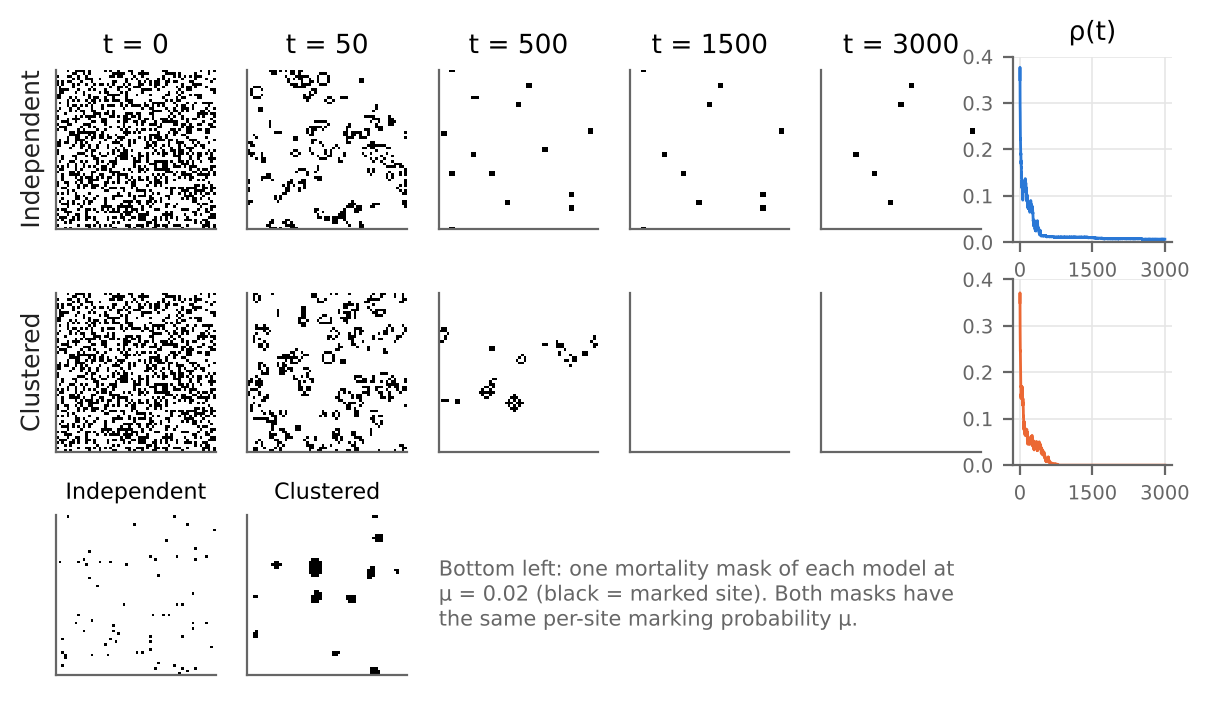
\includegraphics[width=\textwidth]{fig1_snapshots.png}
\caption{Example runs at $\mu=0.005$, $L=60$, $p_0=0.35$ from the same initial grid. Top: independent mortality leaves a sparse population of blocks that survives to $t=3000$. Middle: clustered mortality ($\sigma=2$) extinguishes the population before $t=1000$. Bottom left: one mortality mask of each model at $\mu=0.02$. Both masks mark each site with probability $\mu$.}
\label{fig:snap}
\end{figure}

\subsection{Independent mortality (Experiment A)}

Table~\ref{tab:sweep} and Fig.~\ref{fig:sweep} summarise the sweep. Without mortality the late density at $T=800$ is $0.049\pm0.019$ (mean $\pm$ SD over runs). It falls steeply for small $\mu$. Under independent mortality no run went extinct within 3000 updates for $\mu\le0.005$, extinction became common between $\mu=0.0075$ (4/40) and $\mu=0.015$ (31/40), and all runs went extinct for $\mu\ge0.03$. The surviving populations at $\mu\ge0.002$ were classified as static in every case. They consist of still lifes that are occasionally damaged and repaired, while oscillators did not persist. Late-time activity is therefore close to zero at $\mu>0$ even when the density is positive.

The averaging window has little influence. At $T=3000$, changing $W$ from 50 to 500 changes the mean late density by less than 5\% except near $\mu=0.01$ (about 15\%), where some runs are still declining. Variability is dominated by differences between runs rather than by fluctuations in time. At $\mu=0.005$ the mean within-run temporal SD of $\rho$ over the last 50 states is $1.1\times10^{-4}$, while the SD of the window means across runs is $2.6\times10^{-3}$.

\begin{table}[t]
\centering\footnotesize\setlength{\tabcolsep}{4pt}
\caption{Selected results of Experiment A ($L=60$, $p_0=0.35$, 40 runs per row). $\bar\rho$: mean late density $\pm$ SD across runs. $\bar a$: mean activity over the last 50 updates. $f/\mu$: realised mortality fraction relative to $\mu$. The full table is in \texttt{results/tables/expA\_B\_E\_sweep\_summary.csv}.}
\label{tab:sweep}
\begin{tabular}{llccccrc}
\toprule
Model & $\mu$ & $\bar\rho$ ($T{=}800$, $W{=}160$) & $\bar\rho$ ($T{=}3000$, $W{=}50$) & $\bar a$ & Extinct & Median $\tau$ & $f/\mu$\\
\midrule
Independent & 0 & 0.0494 $\pm$ 0.0190 & 0.0296 $\pm$ 0.0077 & 0.00945 & 0/40 & $>3000$ & -- \\
Independent & 0.001 & 0.0301 $\pm$ 0.0185 & 0.0090 $\pm$ 0.0030 & 0.00005 & 0/40 & $>3000$ & 1.008 \\
Independent & 0.002 & 0.0165 $\pm$ 0.0114 & 0.0088 $\pm$ 0.0032 & 0.00003 & 0/40 & $>3000$ & 0.994 \\
Independent & 0.005 & 0.0101 $\pm$ 0.0051 & 0.0065 $\pm$ 0.0026 & 0.00007 & 0/40 & $>3000$ & 0.992 \\
Independent & 0.01 & 0.0067 $\pm$ 0.0025 & 0.0019 $\pm$ 0.0014 & 0.00004 & 6/40 & $>3000$ & 1.001 \\
Independent & 0.02 & 0.0021 $\pm$ 0.0015 & 0.0000 $\pm$ 0.0002 & 0.00000 & 39/40 & 1130 & 0.995 \\
Independent & 0.05 & 0.0000 $\pm$ 0.0000 & 0.0000 $\pm$ 0.0000 & 0.00000 & 40/40 & 222 & 1.000 \\
\midrule
Control & 0.002 & 0.0206 $\pm$ 0.0178 & 0.0076 $\pm$ 0.0028 & 0.00004 & 0/40 & $>3000$ & 1.001 \\
Control & 0.005 & 0.0110 $\pm$ 0.0079 & 0.0046 $\pm$ 0.0022 & 0.00005 & 0/40 & $>3000$ & 0.997 \\
Control & 0.01 & 0.0064 $\pm$ 0.0024 & 0.0012 $\pm$ 0.0011 & 0.00003 & 13/40 & $>3000$ & 0.995 \\
Control & 0.02 & 0.0013 $\pm$ 0.0012 & 0.0000 $\pm$ 0.0000 & 0.00000 & 40/40 & 954 & 0.995 \\
\midrule
Clustered & 0.001 & 0.0320 $\pm$ 0.0203 & 0.0016 $\pm$ 0.0026 & 0.00038 & 18/40 & $>3000$ & 1.021 \\
Clustered & 0.002 & 0.0191 $\pm$ 0.0152 & 0.0001 $\pm$ 0.0003 & 0.00000 & 37/40 & 1690 & 1.007 \\
Clustered & 0.005 & 0.0034 $\pm$ 0.0062 & 0.0000 $\pm$ 0.0000 & 0.00000 & 40/40 & 841 & 0.996 \\
Clustered & 0.01 & 0.0002 $\pm$ 0.0008 & 0.0000 $\pm$ 0.0000 & 0.00000 & 40/40 & 458 & 0.992 \\
Clustered & 0.02 & 0.0000 $\pm$ 0.0000 & 0.0000 $\pm$ 0.0000 & 0.00000 & 40/40 & 240 & 0.993 \\
\bottomrule
\end{tabular}
\end{table}

\begin{figure}[t]
\centering
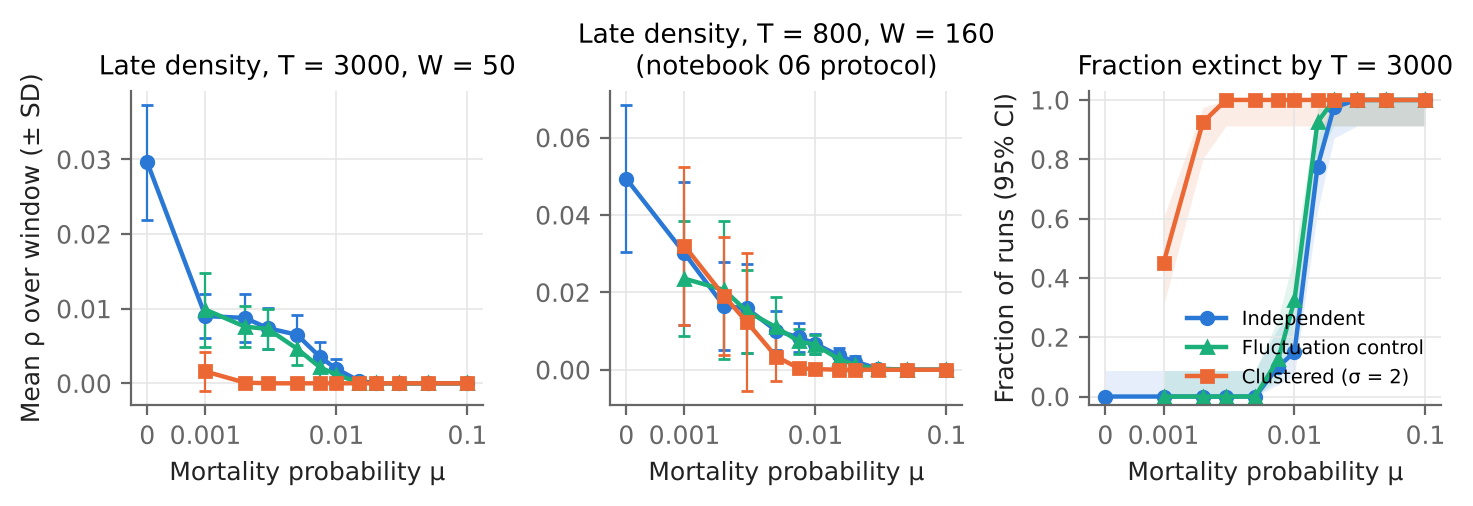
\includegraphics[width=\textwidth]{fig2_mortality_sweep.png}
\caption{Experiment A. Left and centre: mean late density ($\pm$ SD across 40 runs) for two averaging protocols. Right: fraction of runs extinct by $T=3000$ with Wilson 95\% intervals (shaded). The horizontal axis is linear below $\mu=0.001$ and logarithmic above.}
\label{fig:sweep}
\end{figure}

\subsection{Matching of the mortality models (Experiment B)}

The two models are matched in expected mortality. Over 2000 masks on a $60\times60$ lattice the marginal marking probability of the clustered model ($\sigma=2$) is $0.00491\pm0.00009$ for $\mu=0.005$, $0.02016\pm0.00022$ for $\mu=0.02$ and $0.10017\pm0.00056$ for $\mu=0.1$. During the dynamics the realised mortality fraction $f$ lies between $0.985\mu$ and $1.026\mu$ for all 33 conditions of Experiment A (Table~\ref{tab:sweep}, Fig.~\ref{fig:killfrac}a). Because the mask is independent of the configuration, every live cell is exposed to the same probability $\mu$ in both models. The models differ in two respects (Fig.~\ref{fig:killfrac}b). Given that a site is marked, its neighbour is marked with probability 0.67 under clustered mortality ($\sigma=2$, $\mu=0.02$) but 0.02 under independent mortality. In addition, the SD of the marked fraction per update is about four times larger for clustered masks.

\begin{figure}[t]
\centering
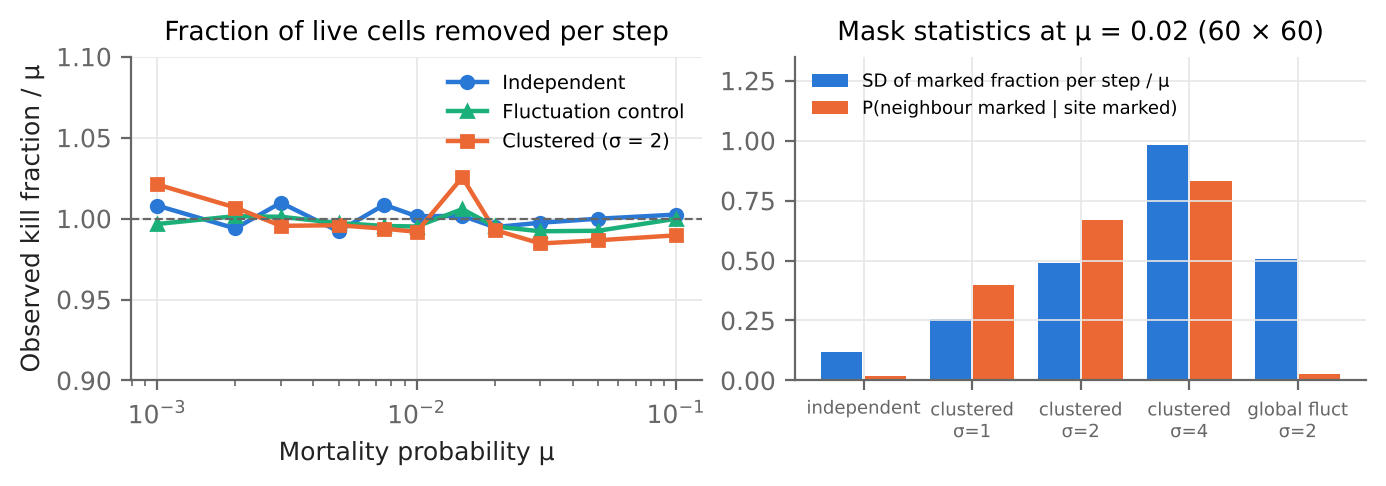
\includegraphics[width=\textwidth]{fig4_mortality_fraction.png}
\caption{Experiment B. (a) Realised fraction of live cells removed per update divided by $\mu$, pooled over 40 runs of $60\times60$ lattices. (b) Two properties of the masks at $\mu=0.02$: the step-to-step SD of the marked fraction (relative to $\mu$) and the conditional probability that a neighbour of a marked site is marked. The control has the fluctuations of the clustered model but not its spatial correlation.}
\label{fig:killfrac}
\end{figure}

\subsection{Clustered mortality and the fluctuation control (Experiments A and F)}

At equal $\mu$, clustered mortality leads to extinction far more often and far sooner than independent mortality (Fig.~\ref{fig:sweep}, right, and Fig.~\ref{fig:survival}). At $\mu=0.005$ all 40 clustered runs went extinct (median $\tau=841$), while none of the 40 independent runs did. Even at $\mu=0.002$, 37 of 40 clustered runs went extinct. The independent model needs a mortality about ten times higher to produce a comparable extinction fraction.

The fluctuation control behaves like the independent model for $\mu\le0.005$ (0/40 extinct). At $\mu=0.01$ it lies in between (13/40, compared with 6/40 independent and 40/40 clustered). Larger fluctuations in the number of deaths therefore contribute somewhat near the extinction threshold of the independent model, but they do not explain the large effect of clustering at low $\mu$.

\begin{figure}[t]
\centering
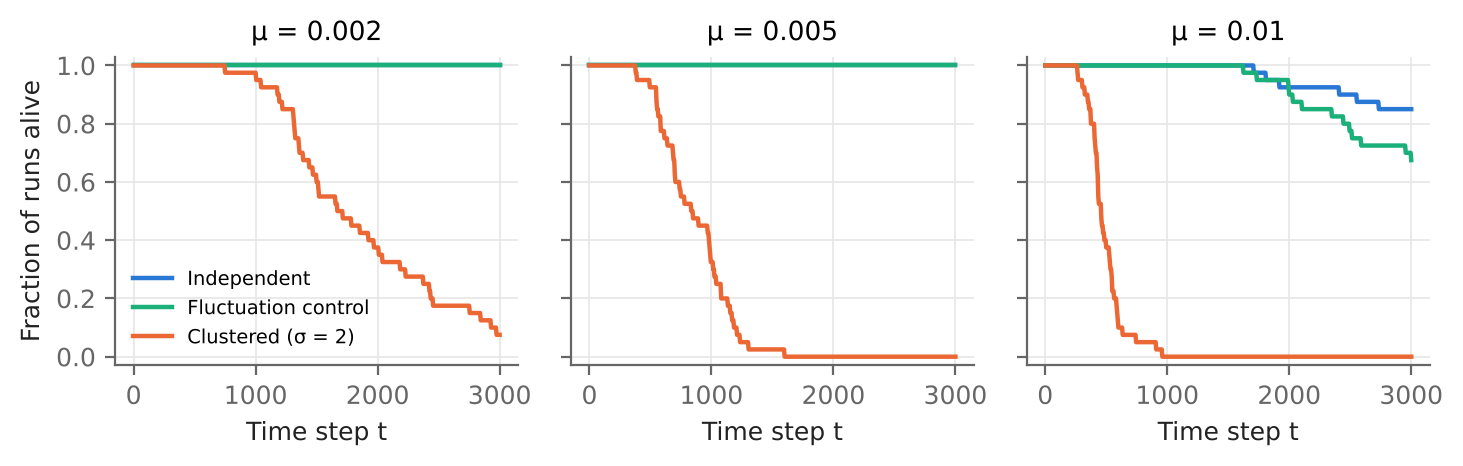
\includegraphics[width=\textwidth]{fig3_survival_curves.png}
\caption{Fraction of runs still alive as a function of time ($L=60$, 40 runs per curve).}
\label{fig:survival}
\end{figure}

The dependence on the correlation width is shown in Fig.~\ref{fig:sigma}. For $\mu\ge0.005$ clustered mortality extinguished every run for $\sigma=1$, 2 and 4. The control approaches the clustered result only for the widest kernel ($\sigma=4$) at $\mu\ge0.01$ (36/40 extinct at $\mu=0.01$). For such wide kernels the number of deaths per update fluctuates strongly (SD comparable to $\mu$ itself), and these fluctuations alone become an important cause of extinction. For $\sigma\le2$ and $\mu\le0.005$ they are not.

\begin{figure}[t]
\centering
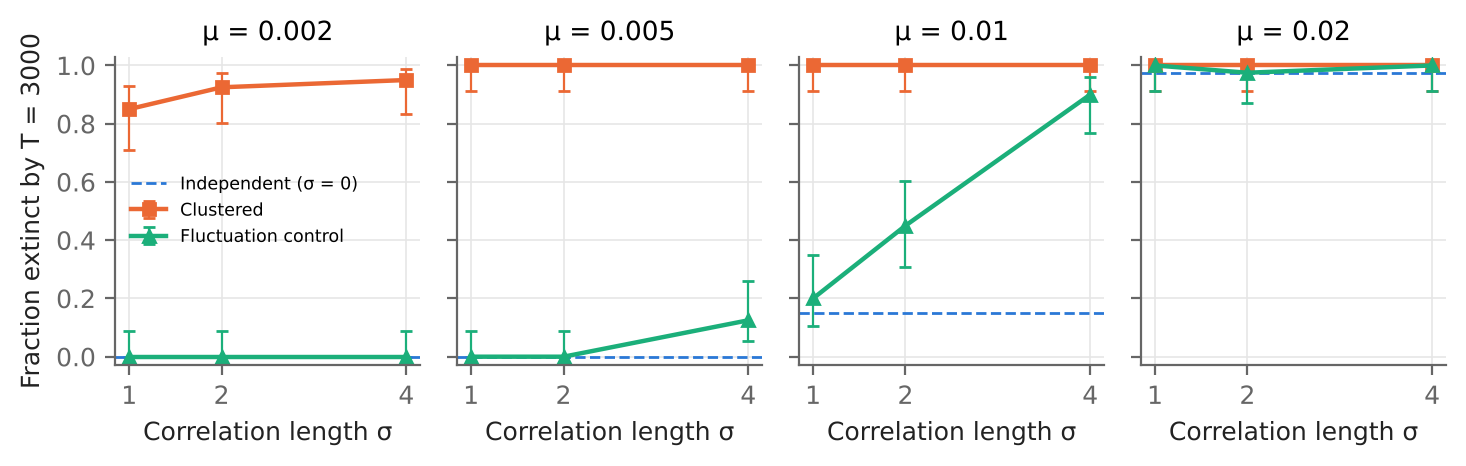
\includegraphics[width=\textwidth]{fig7_sigma.png}
\caption{Experiment F. Fraction extinct by $T=3000$ against the correlation width $\sigma$ for clustered mortality and for the fluctuation control ($L=60$, 40 runs per point, Wilson 95\% intervals). The dashed line is the independent model.}
\label{fig:sigma}
\end{figure}

\subsection{A mechanism: self-repair of still lifes}

The surviving populations at $\mu>0$ consist of still lifes (Experiment E). A $2\times2$ block from which one cell is removed becomes an L-shaped triomino. Its three cells each have two live neighbours and survive, and the empty corner has three and is born, so the block is restored in one update. A block is therefore destroyed only if at least two of its cells are removed in the same update. Under independent mortality this happens with probability of order $6\mu^2$ per update, but under clustered mortality a single event often covers the whole block.

Figure~\ref{fig:objects} tests this directly with isolated objects. At $\mu=0.005$, 252 of 400 isolated blocks survived 3000 updates under independent mortality, whereas the median lifetime under clustered mortality was 124 updates (95\% interval 102 to 138). The control gives an intermediate median of 1093 updates. Objects that are destroyed by a single removal behave in the opposite way. The median lifetime of a beehive was 26 updates under independent and 63 under clustered mortality, and that of a blinker 46 and 70 updates. Clustered marks occur in fewer, larger patches and therefore hit fewer distinct objects. The net effect on a population thus depends on what it consists of. Because the long-lived populations here consist of self-repairing still lifes such as blocks, clustered mortality shortens their lifetime dramatically. This explanation is consistent with all experiments in this report but has not been proven. A census of the surviving objects (Section~\ref{sec:disc}) was made only for one condition.

\begin{figure}[t]
\centering
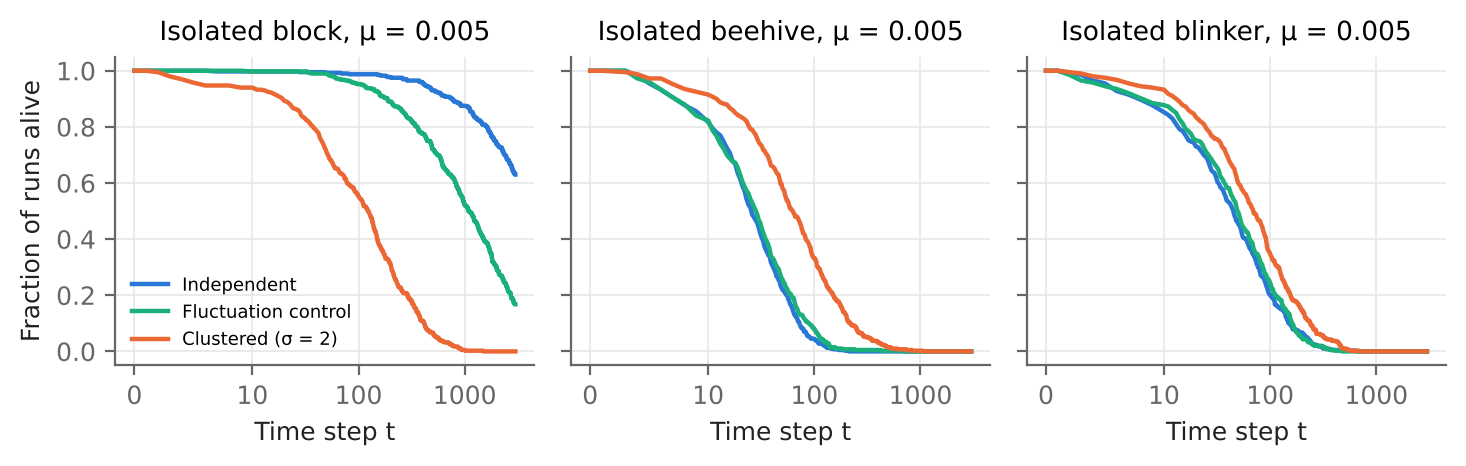
\includegraphics[width=\textwidth]{fig6_object_lifetimes.png}
\caption{Lifetimes of isolated objects on a $32\times32$ torus at $\mu=0.005$ (400 runs per curve). The time axis is linear below 10 and logarithmic above.}
\label{fig:objects}
\end{figure}

\subsection{System size (Experiment C)}

The contrast at $\mu=0.005$ is present at every lattice size (Fig.~\ref{fig:size}). Clustered mortality extinguished all 40 runs for every $L$ from 40 to 200, and independent mortality none for $L\ge60$ (2/40 at $L=40$). Median extinction times increase with $L$ in both models, for example from 647 ($L=40$) to 1335 updates ($L=200$) for clustered mortality at $\mu=0.005$, and from 767 to 2426 for independent mortality at $\mu=0.02$. A larger lattice contains more independent regions, and the whole lattice must die before $\tau$ is reached. The data are compatible with a slow, roughly logarithmic growth of $\tau$ with the number of sites, but no scaling form was fitted and none is claimed. For independent mortality at $\mu=0.02$ and $L=200$ the median extinction time is close to the observation time, so the extinction fraction at $T=3000$ (31/40 here) is sensitive to sampling. The original notebook observed 20/20 for this condition. Forty additional runs with the notebook's own seed formula gave 36/40, which shows that its result was a favourable sample rather than a systematic difference.

\begin{figure}[t]
\centering
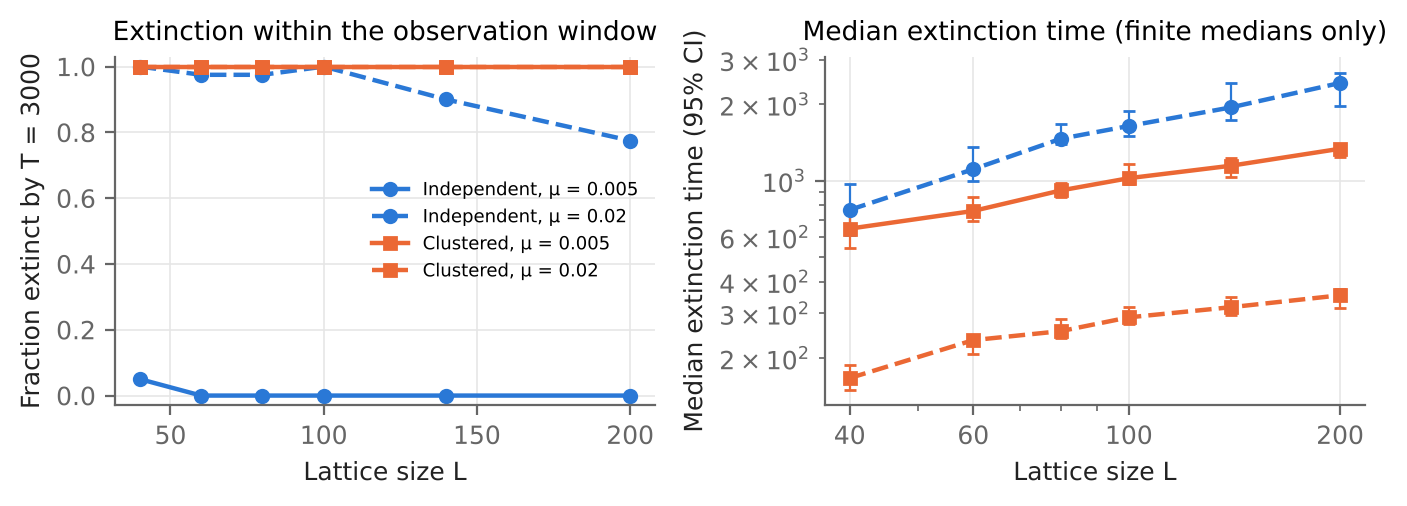
\includegraphics[width=\textwidth]{fig5_system_size.png}
\caption{Experiment C. Left: fraction extinct by $T=3000$. Right: median extinction time with bootstrap 95\% intervals, shown only where at least half of the runs went extinct (40 runs per point).}
\label{fig:size}
\end{figure}

\subsection{Initial conditions (Experiment D)}

The initial density has little effect on the outcome (Fig.~\ref{fig:initial}). For $p_0=0.20$, 0.35 and 0.50 independent mortality at $\mu=0.005$ never led to extinction, and clustered mortality always did. In the nested design (12 initial grids $\times$ 12 mortality seeds), the intraclass correlation, that is the fraction of variance attributable to the initial grid, was between 0 and 0.07 for both the late density and the extinction time. Only one of six $F$-tests gave $p<0.05$ ($p=0.039$), which is not significant after correction for multiple testing. Within this design, the randomness of the mortality process dominates the randomness of the initial condition.

\begin{figure}[t]
\centering
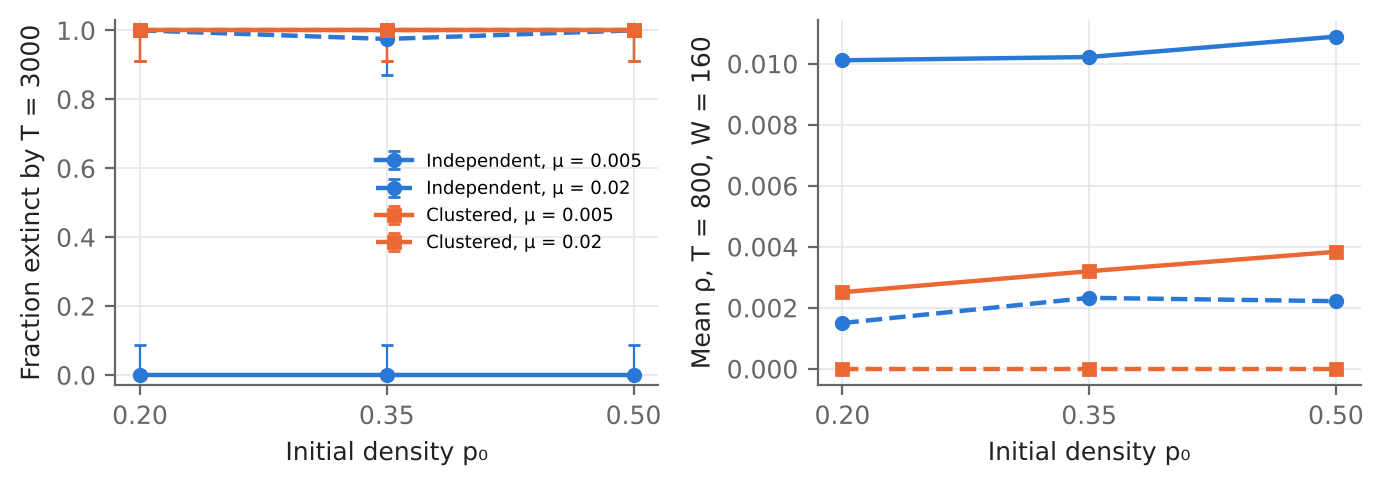
\includegraphics[width=\textwidth]{fig8_initial_density.png}
\caption{Experiment D. Extinction fraction (left, Wilson 95\% intervals) and mean late density at $T=800$ (right) for three initial densities ($L=60$, 40 runs per point).}
\label{fig:initial}
\end{figure}

\section{Statistical analysis}

All comparisons in this report involve differences that are large compared with their uncertainty. For example, at $\mu=0.005$ the extinction fractions 0/40 and 40/40 have non-overlapping Wilson intervals $[0,0.088]$ and $[0.912,1]$. The same holds at every lattice size and every initial density tested. Where a difference is small, such as the location of the late-density maximum in the Week 5 sweep or the $L=200$ extinction fraction discussed above, we have stated that it is not resolved. Extinction times are right-censored at $T=3000$, which is why we report medians and survival curves rather than means. Standard deviations describe variability between independent runs. Standard errors and confidence intervals describe the uncertainty of an estimated mean or fraction. No result in this report depends on a single run.

\section{Discussion}\label{sec:disc}

The central observation of the project, that spatially clustered deaths extinguish the stochastic Game of Life much faster than independent deaths of the same probability, survives every check made here. It is not caused by a difference in mortality strength, which is matched both per site and per live cell. It is not caused by the larger fluctuations in the number of deaths, at least for $\sigma\le2$ and low $\mu$. It does not depend on the lattice size, the initial density or the averaging window within the ranges tested.

The isolated-object experiment points to a simple mechanism. The deterministic Life rule is able to repair small amounts of damage to some still lifes, and blocks dominate the surviving populations. In the 40 independent-mortality runs at $\mu=0.005$, blocks made up 223 of the 241 separate objects (93\%) and 96\% of the live cells at $t=3000$. The remaining objects had one to three cells, consistent with blocks caught in the middle of repair. Independent deaths almost always cause single-cell damage, which the rule repairs. Correlated deaths cause multi-cell damage, which it cannot repair. The same reasoning predicts that clustered mortality should \emph{protect} fragile objects that die from a single hit, and this was observed for the beehive and the blinker. The fate of a population under correlated noise therefore depends on the error-correcting ability of the structures it contains.

\paragraph{Relation to previous work.} Stochastic variants of the Game of Life have been studied with a ``temperature'' \cite{schulman1978}, with probabilistic rules that show transitions between living and extinct phases \cite{monetti1995,nordfalk1996}, with random partial updating \cite{blok1999}, with probabilistic death of cells that violate the survival rule \cite{yaroslavsky2013}, and with rare spontaneous flips of single cells \cite{vidunas2025}. In all of these the randomness acts independently on each site. A preliminary literature search found no study of the Game of Life with spatially correlated mortality, but the search was not systematic and such work may exist. The general effect, however, is well known in spatial ecology. Lattice and metapopulation models show that spatially aggregated disturbances increase extinction risk compared with randomly placed disturbances of the same overall rate \cite{kallimanis2005,liao2015}. Our result is therefore best described as a Game of Life instance of a known ecological phenomenon. What this report adds is a mortality model that is matched exactly in per-cell intensity, a control that separates spatial correlation from fluctuations in the number of deaths, and a specific microscopic mechanism (the self-repair of still lifes) that is particular to the Life rule. That the self-repair of the block is known in the Life community is not in question. The point here is its consequence for the population under correlated noise. The present model, with its absorbing empty state and mortality applied after a deterministic update, is also a natural candidate for the language of absorbing-state transitions \cite{hinrichsen2000}. With the lattice sizes and observation times used here we do not claim to have located a phase transition.

\section{Limitations}

\begin{itemize}
\item Lattices are finite ($L\le200$) and observation times are finite ($T\le3000$). Survival up to $T$ does not imply survival forever, and on a finite lattice every run eventually goes extinct.
\item Most conditions use 40 runs, which gives extinction fractions with 95\% intervals of up to about $\pm0.15$.
\item Only one form of spatial correlation (a Gaussian kernel) and three widths were studied. Temporal correlations of the noise were not considered.
\item The fluctuation control removes spatial correlation while keeping fluctuations in the global death rate. Other controls are possible.
\item The long-time labels rely on operational thresholds (30-update settling time, comparison 300 updates apart) whose influence was not studied.
\item The mechanism is supported by isolated-object simulations and by a census of surviving objects for one condition (independent mortality, $\mu=0.005$, $L=60$). Other conditions were not counted.
\item The literature search was preliminary. The connection to the ecological literature on spatially correlated disturbance should be developed further.
\end{itemize}

\section{Conclusions}

In the stochastic Game of Life with mortality probability $\mu$, the spatial arrangement of deaths has a strong effect on the long-time fate of the system. At $\mu=0.005$, independent deaths never extinguished a $60\times60$ population within 3000 updates, whereas clustered deaths with the same per-cell probability always did. This contrast does not result from a difference in average mortality and, for moderate correlation widths, not from fluctuations in the number of deaths. It holds for all lattice sizes and initial densities tested. A plausible mechanism is that clustered deaths defeat the self-repair of still lifes such as the block. Natural next steps are a census of the surviving structures under more conditions, longer runs and larger samples near the extinction threshold, a systematic study of the correlation width, and a comparison with the literature on stochastic Life and absorbing-state transitions.

\section*{Reproducibility information}

All code, data and figures are in the repository \url{https://github.com/yildizaliyigit067-dotcom/CA} (branch \texttt{main}). The results were produced with Python 3.13.18, NumPy 2.5.3, SciPy 1.18.1, pandas 3.0.5, Matplotlib 3.11.2 and Numba 0.68.1 on a two-core Linux machine. The commands
\begin{verbatim}
python -m pytest analysis/tests -q
python analysis/experiments.py all
python analysis/make_figures.py
python analysis/crosscheck_nb06.py
\end{verbatim}
regenerate every number and figure in this report in about 25 minutes. Each row of the run-level CSV files records the \texttt{SeedSequence} keys of its initial grid and of its mortality process. The notebooks \texttt{01} to \texttt{06} run from top to bottom and reproduce their stored outputs.

\section*{Statement on the use of AI}

AI tools (Claude and ChatGPT) were used during the weekly project as recorded in \texttt{AI\_NOTES.md}. The English translation of the notebooks, the verification code in \texttt{analysis/}, the additional simulations and the text of this report were produced with the help of Claude (Anthropic) in November 2026. The research question, the original model, the choice of the clustered-death comparison and the original experiments are the student's.

\begin{thebibliography}{99}\small
\bibitem{bak1989} P.~Bak, K.~Chen and M.~Creutz, Self-organized criticality in the `Game of Life', \emph{Nature} \textbf{342}, 780--782 (1989). doi:10.1038/342780a0
\bibitem{bennett1991} C.~Bennett and M.~S.~Bourzutschky, `Life' not critical?, \emph{Nature} \textbf{350}, 468 (1991).
\bibitem{blok1999} H.~J.~Blok and B.~Bergersen, Synchronous versus asynchronous updating in the ``game of Life'', \emph{Phys. Rev. E} \textbf{59}, 3876--3879 (1999). doi:10.1103/PhysRevE.59.3876
\bibitem{efron1979} B.~Efron, Bootstrap methods: another look at the jackknife, \emph{Ann. Statist.} \textbf{7}, 1--26 (1979).
\bibitem{gardner1970} M.~Gardner, Mathematical Games: The fantastic combinations of John Conway's new solitaire game ``life'', \emph{Scientific American} \textbf{223}(4), 120--123 (1970).
\bibitem{harris2020} C.~R.~Harris \emph{et al.}, Array programming with NumPy, \emph{Nature} \textbf{585}, 357--362 (2020).
\bibitem{hinrichsen2000} H.~Hinrichsen, Non-equilibrium critical phenomena and phase transitions into absorbing states, \emph{Adv. Phys.} \textbf{49}, 815--958 (2000). doi:10.1080/00018730050198152
\bibitem{kallimanis2005} A.~S.~Kallimanis \emph{et al.}, Metapopulation extinction risk under spatially autocorrelated disturbance, \emph{Conserv. Biol.} \textbf{19}, 534--546 (2005). doi:10.1111/j.1523-1739.2005.00418.x
\bibitem{liao2015} J.~Liao, Z.~Ying, D.~E.~Hiebeler, Y.~Wang, T.~Takada and I.~Nijs, Species extinction thresholds in the face of spatially correlated periodic disturbance, \emph{Sci. Rep.} \textbf{5}, 15455 (2015). doi:10.1038/srep15455
\bibitem{vidunas2025} R.~Vidunas and A.~Vaicekauskas, Conway's game ``Life'' perturbed, arXiv:2503.19869 (2025).
\bibitem{yaroslavsky2013} L.~P.~Yaroslavsky, The amazing dynamics of stochastic pattern formation and growth models inspired by the Conway's Game of Life, arXiv:1304.8104 (2013).
\bibitem{lam2015} S.~K.~Lam, A.~Pitrou and S.~Seibert, Numba: a LLVM-based Python JIT compiler, in \emph{Proc. Second Workshop on the LLVM Compiler Infrastructure in HPC} (2015).
\bibitem{martin1984} O.~Martin, A.~M.~Odlyzko and S.~Wolfram, Algebraic properties of cellular automata, \emph{Commun. Math. Phys.} \textbf{93}, 219--258 (1984). doi:10.1007/BF01223745
\bibitem{monetti1995} R.~A.~Monetti and E.~V.~Albano, Critical edge between frozen extinction and chaotic life, \emph{Phys. Rev. E} \textbf{52}, 5825--5831 (1995). doi:10.1103/PhysRevE.52.5825
\bibitem{nordfalk1996} J.~Nordfalk and P.~Alstr{\o}m, Phase transitions near the ``game of Life'', \emph{Phys. Rev. E} \textbf{54}, R1025--R1028 (1996). doi:10.1103/PhysRevE.54.R1025
\bibitem{schulman1978} L.~S.~Schulman and P.~E.~Seiden, Statistical mechanics of a dynamical system based on Conway's game of Life, \emph{J. Stat. Phys.} \textbf{19}, 293--314 (1978). doi:10.1007/BF01011727
\bibitem{virtanen2020} P.~Virtanen \emph{et al.}, SciPy 1.0: fundamental algorithms for scientific computing in Python, \emph{Nat. Methods} \textbf{17}, 261--272 (2020).
\bibitem{wilson1927} E.~B.~Wilson, Probable inference, the law of succession, and statistical inference, \emph{J. Am. Stat. Assoc.} \textbf{22}, 209--212 (1927).
\bibitem{wolfram1983} S.~Wolfram, Statistical mechanics of cellular automata, \emph{Rev. Mod. Phys.} \textbf{55}, 601--644 (1983). doi:10.1103/RevModPhys.55.601
\bibitem{wolfram1984} S.~Wolfram, Universality and complexity in cellular automata, \emph{Physica D} \textbf{10}, 1--35 (1984).
\end{thebibliography}

\appendix
\section{Corrections made to the project notebooks}

During the review one execution-order bug in notebook~06 was fixed (a loop variable overwrote a test grid), the population of the toad oscillator in notebook~04 was corrected from ``6 to 8'' to 6, and several statements were annotated where the data did not support them. No model, parameter or stored result was changed. Details are in \texttt{VALIDATION\_REPORT.md} and \texttt{CHANGELOG.md}.

\end{document}
